\chapter{THEORETICAL BACKGROUND}
\label{chap3:background}

The theoretical background defines a variety of subjects, including traditional machine learning methods, deep learning methods, federated learning concepts for training the model to classify the cervical cell images and other relevant concepts.

\section{Traditional Machine Learning Algorithms}

\subsection{LightGBM}
Light Gradient Boosting Machine or, LightGBM is a highly efficient Gradient boosting decision tree, which provides increased accuracy and efficiency. It is a gradient boosting framework that utilizes tree based learning algorithms. It has the advantages like capability of handling larger scale data, better accuracy, decreased memory usage, etc. LightGBM splits the tree leaf-wise in order to ensure lower loss. 

\begin{figure}[H]
\centering
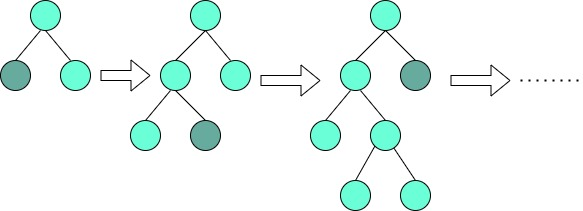
\includegraphics[width=150mm,height=50mm]{figures/lgbm.jpg}
\caption{Leaf-wise tree growth used in LightGBM}
\label{DLAccuracy}
\end{figure}


The LightGBM algorithm utilizes two novel techniques called Gradient-Based One-Side Sampling (GOSS) and Exclusive Feature Bundling (EFB) which allow the algorithm to run faster while maintaining a high level of accuracy \cite{ar22}.

\subsection{Histogram Gradient Boosting With LightGBM}
In order to speed up the Gradient boosting decision tree (GDBT) process,using histogram proves to be an important technique \cite{ar23}. To ensure better quality in less inference time, an advanced base learner called piecewise linear tree is utilized.

\begin{figure}[H]
\centering
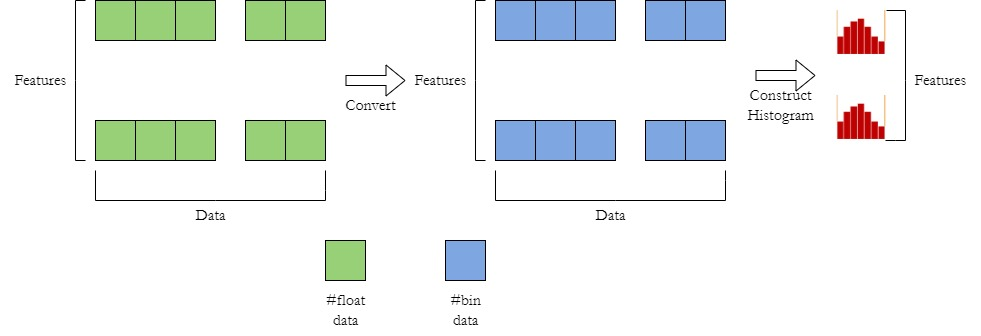
\includegraphics[width=160mm,height=55mm]{figures/hgb_lgbm.jpg}
\caption{Histogram Algorithm of LightGBM}
\label{DLAccuracy}
\end{figure}

\subsection{Histogram Gradient Boosting}
Histogram Boosting was released by Scikit-Learn, which was named as HistGradientBoostingClassifier. Its operation is similar to that of LightGBM, but offers a much faster speed than gradient boosting. It provides built in support for the missing values, and is used for faster training of decision trees.  

\subsection{Xtra Trees}
Extremely randomized trees or extra trees is an ensemble supervised machine learning method. The extra trees algorithm works by creating multiple decision trees, where the sampling for each tree is done randomly. Thus the dataset taken for each tree is made with unique samples. To output the classification result, it aggregates the results of the multiple de-correlated decision trees, which are collected in a "forest". Thus it holds similarity to the Random Forest Classifier, but differs with respect to the construction of the Decision Trees in the forest.

\subsection{SVM}
Support Vector Machine (SVM) is a machine learning method which helps to largely overcome the curse of dimensionality and other issues faced while applying the traditional learning methods. SVM takes the optimal separating hyperplane as the decision surface, which is able to classify two classes of data while maximizing the distance between the points \cite{ar24}.  Thus all of the data points on one side of the hyperplane will represent one category and the data points on the other side of the hyperplane will represent a different category. Support vector machines are a set of supervised learning methods, that can be used to detect cancerous cells, on the basis of millions of cells.

\subsection{SVM Grid Search}
SVM has some hyper-parameters, and the optimal one can be found by creating a grid of hyper-parameters and just try all the possible combinations. This approach taken is termed as Grid Search. In the Grid Search method, all the possible combinations of hyperparameters will pass one by one into the model and check each model's score. As a result, it gives us a set of hyperparameters which give the best possible score.  Grid Search calculates the error for various hyperparameter values, and eventually aids in choosing the best values.

\subsection{Gradient Boosting}
Gradient boosting is a machine learning technique that is used in both regression and classification tasks. It gives a prediction model in the form of an ensemble of weak prediction models, which are typically decision trees. It is termed as a sequential ensemble learning technique, as the performance of the model is found to improve over iterations. In this case a group of weak prediction models, like regression decision trees, are modeled by adding new learners in a sequential manner. It can give prediction results based on the decision nodes, and can provide an improved accuracy when viewed as an ensemble \cite{ar25}. 

\subsection{XGBOOST}
Extreme Gradient Boosting or XGBoost also uses a gradient-boosting based approach in order to ensure optimization in the tree split against a predefined loss function.  It is an ensemble learning method which combines the predictions of multiple weak models to produce a stronger prediction. XGBoost has the advantage that it can deal with any missing data, unlike other ML models that require additional processing on the training data. It does not require an immense set of pre-processing operations and thus minimizes the communication costs significantly and also reduces the leakage of  private data \cite{ar26}. 

\begin{figure}[H]
\centering
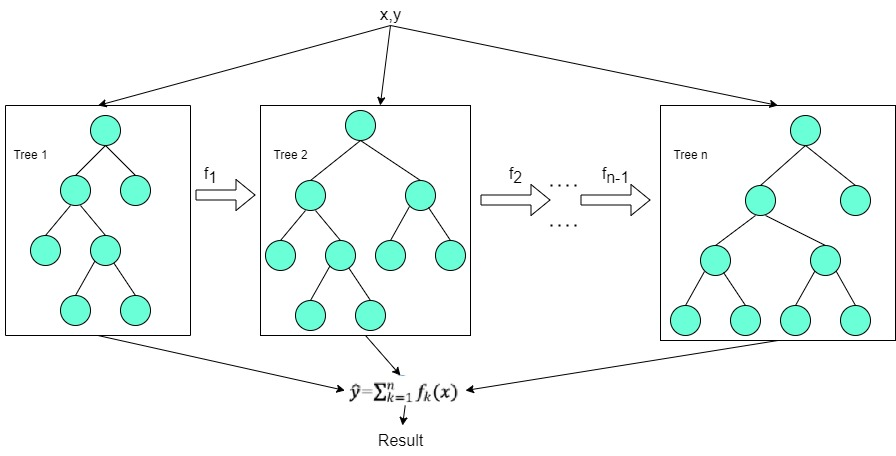
\includegraphics[width=150mm,height=70mm]{figures/xgb.jpg}
\caption{A General Architecture of XGBoost}
\label{DLAccuracy}
\end{figure}

XGBoost has a wide range of hyperparameters that can be adjusted to optimize performance, making it highly customizable and also provides feature importances, which helps in making important predictions.

\subsection{MLP}
A multilayer perceptron (MLP) is a fully connected class of feedforward artificial neural network (ANN). The multilayer perceptron can be trained to approximate virtually any measurable function, as it does not make any prior assumption regarding the data distribution. The multilayer perceptron can model the non-linear functions, and can also be trained so that whenever presented with any unseen data, it can accurately generalise the information \cite{ar28}. The multilayer perceptron is a system of interconnected neurons, consisting of input and output layers, and one or more hidden layers.

\begin{figure}[H]
\centering
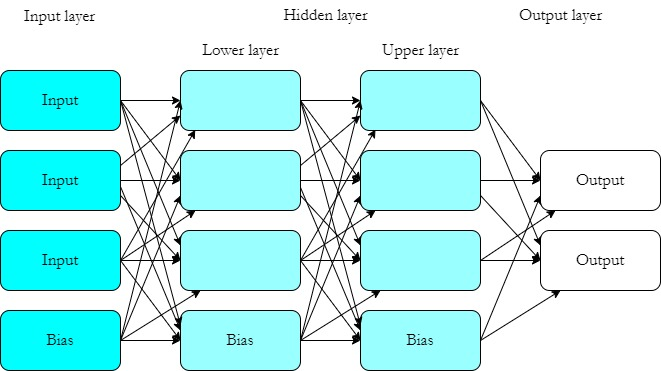
\includegraphics[width=125mm,height=70mm]{figures/mlp.jpg}
\caption{The multilayer perceptron}
\label{DLAccuracy}
\end{figure}

\subsection{Histogram Gradient Boosting With XGBoost}
Histograms can be applied to the Extreme Gradient Boosting, or XGBoost for the continuous input variables. It eventually helps to provide a highly optimized implementation of gradient boosting.

\subsection{KNN}
K-Nearest Neighbor or KNN Algorithm is a non-parametric, supervised learning classifier, which makes use of approximation to make classifications about the grouping of an individual data point. It can be used for both regression and classification, but it is mostly utilized in classification algorithms. The average of the k nearest neighbors is considered to make a prediction about the classification of a new data point. For this, the K-NN algorithm assumes the similarity between the new data and all the available data and places the new data into the category which is most similar to the available categories.

\begin{figure}[H]
\centering
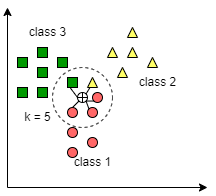
\includegraphics[width=95mm,height=75mm]{figures/knn.png}
\caption{K Nearest Neighbours}
\label{DLAccuracy}
\end{figure}

KNN is a non-parametric algorithm, as it does not make any assumption regarding the underlying data. It is sometimes termed as a lazy-learner as it does not learn anything from the training set immediately. It merely stores the dataset and performs an action on it at the time of classification.


\subsection{Decision Tree}
A decision tree is a decision support tool that uses a tree-like model, made up of decisions and their possible consequences. An instance is classified by starting at the root node of the tree, then it gradually moves down until it reaches the leaf. The internal nodes denote a test on an attribute. Drawn from left to right, the contents of the leaf node represent the outcome of the decisions. The decision tree follows a non-parametric approach, which means that it is distribution-free and does not depend on the assumptions of probability distribution. It can operate on any high-dimensional data with exceptional accuracy.

\begin{figure}[H]
\centering
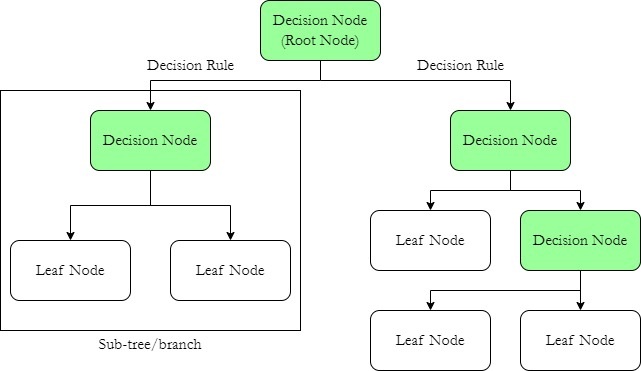
\includegraphics[width=130mm,height=80mm]{figures/dt.jpg}
\caption{Decision Tree Classifier}
\label{DLAccuracy}
\end{figure}

\subsection{AdaBoost}
AdaBoost or Adaptive Boosting is a method in machine learning, which is used as an ensemble learning  method. A strong model can be built by grouping multiple weak classifiers where each one gets to progressively learn from the others' wrongly classified objects. The multiple weaker models are independently trained and their predictions get combined to make the overall prediction.

% \begin{figure}[H]
% \centering
% 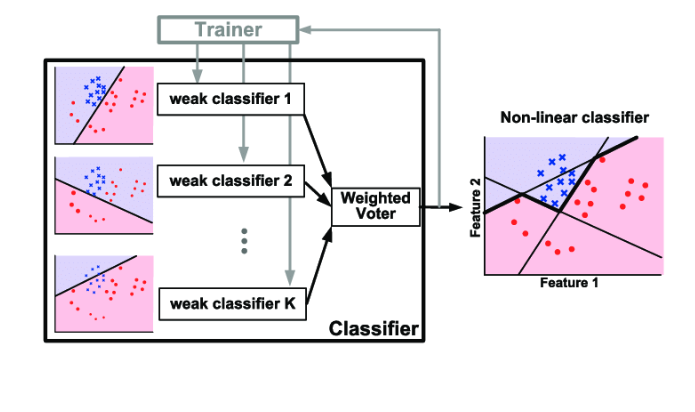
\includegraphics[width=90mm,height=38mm]{figures/adaboost.png}
% \caption{AdaBoost algorithm for creating a strong classifier based on multiple weak linear classifiers.}
% \label{DLAccuracy}
% \end{figure}

% The application of  algorithms in order to create a strong classifier is shown in fig …. 

Boosting is a machine learning technique used for both regression and classification problems. It produces a prediction model which holds characteristics which represent an ensemble of weak prediction models, typically decision trees. It builds the model in a gradual manner, like other boosting methods do. It generalizes the models by allowing optimization of an arbitrary differentiable loss function (\cite{ar27}).

\subsection{Random Forest}
are ensemble learning techniques for classification, regression, and other problems that work by building a large number of decision trees during the training phase The class most trees choose in a classification problem is the output of the random forest.

\subsection{Gaussian Naive Bayes}
It is an extension of the Naive Bayes Algorithm. Gaussian Naive Bayes is a classification technique, which is used in Machine Learning (ML) based on the probabilistic approach and Gaussian distribution. This algorithm does not need much time for training and gives results which are greatly reliable. 

\section{Deep Learning}
Artificial neural networks, a class of algorithms inspired by the structure and operation of the brain, are the focus of the machine learning discipline known as deep learning. Some of the data pre-processing that is generally involved with machine learning is eliminated with deep learning. These algorithms can handle text and visual data that is unstructured and automate feature extraction, reducing the need for human specialists. 

The process of recognizing photographs and classifying them into one of several predetermined different categories is known as image recognition (or image classification). As a result, image recognition software and apps can identify the objects in a photo and differentiate one from another. Computer vision is the branch of study that aims to give machines this capability. Deep learning models can be used by researchers to solve computer vision problems.

Deep learning systems need access to enormous amounts of training data and processing power in order to attain an acceptable degree of accuracy. Until the age of big data and cloud computing, neither of these resources was readily available to programmers. Deep learning is able to produce precise predictive models from enormous amounts of unlabeled, unstructured data because it is capable of producing complicated statistical models directly from its own iterative output. 

\subsection{CNN}
A Convolutional Neural Network (ConvNet/CNN) is a Deep Learning algorithm that can take in an input image, give importance (learnable weights and biases) to various aspects in the image, and be able to distinguish one from the other. In comparison to other classification methods, a ConvNet requires significantly less pre-processing. ConvNets have the capacity to learn these filters and properties, whereas in basic techniques filters are hand-engineered.

The structure of a ConvNet was influenced by the way the Visual Cortex is organized and is similar to the connectivity pattern of neurons in the human brain.

\subsection{Layers of CNN}
Convolutional Neural Networks (CNNs) are constructed from layers that perform different operations on the input data. The primary layers used to construct a CNN are as follows:

\subsubsection{Convolutional layer}
To perform the convolution process, a convolutional layer applies a number of learnable filters or kernels to the input image or feature map. A set of feature maps that represent different aspects of the input picture or feature map make up a convolutional layer's output. Let K be the kernel detector and I be the image used as the input. The output feature map O can then be created by convolving the input image with the kernel and using an activation function, similar to what was done in 3.1:

\begin{equation}
\label{eq:cnn_conv_layer}
    \textcolor{black}{O(i,j) = f(\sum\sum I(m,n) * K(i-m,j-n)}
\end{equation}

where f denotes the activation function, (i,j) denotes a location in the output feature map, and (m,n) denotes the location of the input image pixel that the kernel is now aligned with. The whole feature map can be retrieved by swiping the kernel over the full input image.

\subsubsection{Activation Layer}
An activation layer applies a non-linear activation function to the output of a fully connected layer or a convolutional layer.

Let X be the input (which is often the output of a convolutional or fully connected layer) and f be the activation function for the activation layer. Each element of the input X is subjected to the activation function by the activation layer, which results in the output Y. As seen below, the output Y is calculated:

\begin{equation}
\label{eq:activation_layer}
    \textcolor{black}{Y(i,j,c) = f(X(i,j,c)}
\end{equation}

where i, j, and c are the input and output tensors' spatial and channel coordinates. Sigmoid, tanh, and ReLU (Rectified Linear Unit) activation functions are frequently used in CNNs. The precise requirements of the work and the type of data being processed dictate the activation function to be used.

\subsubsection{Pooling Layer}
A pooling layer reduces the spatial size of feature maps while retaining the most crucial data. The two most used pooling operations are average pooling, which chooses the average value from each patch of a feature map to produce a smaller map, and max pooling, which returns the maximum value inside a pooling window. The following mathematical diagram illustrates how pooling works:
Let P represent the pooling size, S represent the stride, and F represent the input feature map. The output feature map O can then be created by pooling the input feature map with a pooling window of size P and a stride of S:

\begin{equation}
\label{eq:pooling_layer}
    \textcolor{black}{O(i,j) = Pooling(F(iS : iS+P,jS : jS+P)}
\end{equation}

% O(i,j) = Pooling( F(iS : iS+P, jS : jS+P) )

where Pooling is a pooling function that produces a single value from values in the pooling window.

\subsubsection{Batch Normalization Layer}
The layer of batch normalization enables the network's layers to learn more independently. The output of the earlier layers is normalized using it. In normalization, the activations scale the input layer. Learning becomes more effective when batch normalization is utilized, and it can also be used as regularization to prevent model overfitting. To standardize the input or the output, the layer is added to the sequential model. It can be applied in a number of places between the model's layers. It is frequently positioned immediately after the convolution and pooling layers and after specifying the sequential model.

\subsubsection{Dropout}
The regularization method used to stop overfitting in the model is called dropouts. A certain percentage of the network's neurons are switched at random with the addition of dropouts. The incoming and outgoing connections to the neurons are also turned off when they are turned off. To help the model learn more effectively, this is done. Dropouts are typically advised against using them after convolution layers; instead, they should be utilized after the network's dense layers. It is always advisable to turn off the neurons just to 50\%. There is a possibility that the model leaning and the forecasts would be poor if we turned off more than 50\%.

\subsubsection{Flatten Layer}
A flattened layer transforms a 2D or 3D feature map into a 1D vector that can be used as input to fully connected layer. 
Let F be the input feature map of size H x W x C, where H is the height, W is the width, and C is the number of channels. Concatenating the rows of the feature map will then yield the flattened vector F':

\begin{equation}
\label{eq:flatten_layer}
    \textcolor{black}{F' = [F(1,1,1), F(1,2,1), ..., F(1,W,1), F(2,1,1), ..., F(H,W,1), F(1,1,2), ..., F(H,W,C)]}
\end{equation}

% F' = [F(1,1,1), F(1,2,1), ..., F(1,W,1), F(2,1,1), ..., F(H,W,1), F(1,1,2), ..., F(H,W,C)]

where the value of the feature map at position (i,j) in channel c is represented by F(i,j,c). The 2D or 3D feature map is flattened into a 1D vector using the equation above, which may then be utilized as input to a fully connected layer or other kinds of layers in the neural network.

\subsubsection{Fully Connected Layer}
The flattened feature vector serves as the fully connected layer's input, and a group of class scores serves as its output. Neurons in the layer that is entirely interconnected are coupled to each and every neuron in the layer below it. Generally, the output of the fully connected layer is fed into a softmax layer, which converts class scores into a probability distribution across classes.

\subsection{Activation Function}
An activation function is a mathematical function that deep neural networks employ to introduce nonlinearity into a layer's output. The use of activation functions is used to achieve this. It is used to change a layer's output into a more complex representation, allowing the network to learn complex and non-linear relationships between the input and the output. The ReLU activation function is applied following each convolutional layer in any CNN. As a result, the layer's output is effectively made non-linear, allowing the network to learn intricate details from the input images.

The activation functions Sigmoid, Tanh (Hyperbolic Tangent), and Leaky ReLU are frequently employed in deep learning. Based on the features of the data and the nature of the problem being addressed, the activation function is chosen.

\subsubsection{ReLU (Rectified Linear Unit):}
Deep neural networks frequently use the ReLU activation function since research has shown that it enhances the training of deep models. Any negative input is translated to 0, while positive inputs are left unaffected. The ReLU function is described as:

\begin{equation}
\label{eq:relu}
    \textcolor{black}{f(x) = max(0, x)}
\end{equation}
% $f(x) = max(0, x)$
The activation function's input in this case is 'x'. The ReLU function's output is almost always non-negative. The ReLU function's output is equal to the input when the input is positive. The output of the ReLU function is zero when the input is negative. ReLU is frequently used as the activation function in a neural network's hidden layers, while sigmoid is frequently utilized as the activation function in the output layer for binary classification tasks.

\subsubsection{Sigmoid:} 
For binary classification tasks, the sigmoid activation function is frequently used. All real-valued input is converted to a value between 0 and 1, which can be thought of as a probability. The sigmoid function is described as:

\begin{equation}
\label{eq:sigmoid}
    \textcolor{black}{f(x) = \frac{1}{(1+e^{-x})}}
\end{equation}
% $f(x) = \frac{1}{1+e^{x}}$
In this case, the activation function's input is 'x'. The sigmoid function's output has an inflection point at x = 0, and it always ranges between 0 and 1. The sigmoid function's output gets closer to one when the input is positive. The output of the sigmoid function gets closer to zero when the input is negative.


\section{Federated Learning}
\subsection{Federated Learning Mechanism}
Federated Learning is a collaborative machine learning technique where multiple edge devices(clients) participate remotely to train a common, robust machine learning model (server) without exchanging/sharing their local data samples with the centralized location or server which helps organizations to make better decisions with AI, addressing critical issues of data privacy, security, access rights and access to heterogeneous data.

\subsection{Traditional ML Vs. Federated Learning}
Traditional machine-learning approaches require a centralized location i.e. a single server to aggregate user data and carry out the complete training process, whereas federated learning allows continuous training on edge devices while ensuring no sensitive information exits the device. In the classical machine learning model, it is quite common to assume that the data are independent and identically distributed. On the contrary, federated learning assumes the data to be non-i.i.d because in real-world circumstances, various users have different datatypes and the expected and actual number of actors varies.

\subsection{Data Partitioning}
There are 3 types of data partitioning systems in federated learning: horizontal data partitioning, vertical data partitioning and federated transfer learning system. The description of the these 3 types is given below:

\textbf{1. Horizontal Data Partitioning :}
In horizontal partition, each edge device has overlapping features with different observations. For instance, if multiple hospitals in various countries collect data on breast cancer patients but have little to no overlapping of patients, that distribution is horizontal partitioning \cite{ar17}. 
		
\textbf{2. Vertical Data Partitioning :}
In the vertical partition, each device has different features with overlapping observations. For example, if a hospital suggests patients to a specific surgeon, both the hospital and the surgeon collect different kinds of data but will have many common patients \cite{ar17}.

\textbf{3. Federated Transfer Learning :}
If there are a few similar samples with few similar features, but also samples and features do not overlap, then federated transfer learning can be applied in this situation \cite{ar17}.

\subsection{Foundation ML model}
Depending on real-life scenarios, limitations of available datasets and problem statements, different kinds of ML models are decided to be used as the foundation model of federated learning architecture. Neural networks, decision trees, and even linear models are used on basis of use cases. This base model serves as a global model which is initially distributed as an untrained or pre-trained model from a central server to the local clients. The clients then collaboratively train the global model by continuously improving it in every communication round between the central server and the local clients. 

\subsection{Communication Architecture}
There are two types of FL communication architecture: centralized and decentralized. Both types of architecture work similarly; the distinction between them is in client-server communication. 

\textbf{1. Centralized Federated Learning :}
In a centralized federated learning system, a single central server is used, so there is only one possible point of failure \cite{ar19}.  In a centralized federated learning environment, a central server is utilized to manage all the participating nodes and orchestrate the various steps of the algorithms. The server is in charge of selecting the nodes at the start of the training process and aggregating the received model parameter updates. The server can end up being the system's bottleneck because each of the chosen nodes must communicate updates to the server \cite{ar18}. 

\textbf{2. Decentralized Federated Learning :}
Decentralized federated learning does not rely on a single central server to provide updates, in contrast to centralized federated learning \cite{ar19}. In this architecture, the nodes can collaborate among themselves to produce the global model. As the model updates are solely transferred between linked nodes without the coordination of a central server, this configuration avoids single-point failures \cite{ar21}. 

\subsection{Scale of Federation}
Federated learning can be divided into two categories based on the participating clients and the model training scale: cross-device FL and cross-silo FL \cite{ar20}.

\textbf{1. Cross-silo}: Cross-silo FL, where clients are organizations or companies and the client number is typically low (e.g., within a hundred) \cite{ar20}. 

\textbf{2. Cross-device}: Cross-device, where clients are typically mobile devices and the client number can reach millions \cite{ar20}. 


\subsection{One Federated Round}
The step where each participant completes training their local model and sends their model weights to the server so the server can combine their global model with the recently updated parameters of local models is referred to as a single communication round between the server and participant clients.

\subsection{Participants of the network}

There are two types of participants in a single federated round :
\begin{itemize}
    \item Client devices: These are the local devices that participate in the federated learning process by sending the updated weights of their locally trained models to the server.
    \item Server: The server uses the federated learning process by aggregating the model weights received from the client devices and sending the averaged weights back to the local devices for further training and to improve their accuracy.
\end{itemize}

\subsection{Process}

In a single federated round, the following steps are completed one after another: 
\begin{enumerate}
    \item The client devices obtain the initialized global model from the cloud server.
    \item They train the model using the local datasets and generate the most recent local model update (model parameters).
    \item Then they send the updated weights of their locally trained model to a central server. 
    \item The cloud server collects various local update parameters and aggregates the model weights received from all of the client devices by averaging them together.
    \item The averaged weights are then sent back to the client devices, which use them to train their local models further.
    \item This process is repeated until the models on the client devices reach satisfactory accuracy.
\end{enumerate}

\begin{figure}[H]
\centering
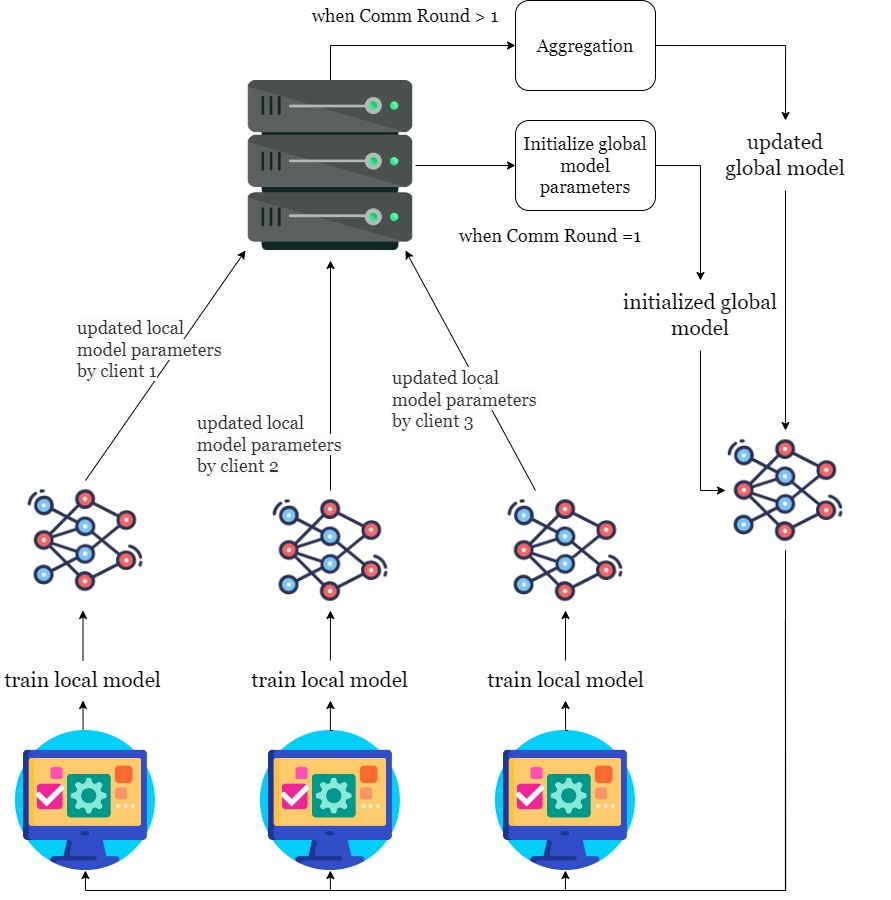
\includegraphics[width=100mm,height=92mm]{figures/federatedround.jpg}
\caption{Flowchart of federated learning}
\label{Flowchart of federated learning}
\end{figure}

\section{Federated Learning training algorithm}
\subsection{FedSGD (Federated Stochastic Gradient Descent)}
Stochastic Gradient Descent (SGD) can be applied to as a base to the Federated Learning training algorithm. A single batch gradient calculation is done on each round of communication. Although this approach is computationally efficient, it requires a large number of training rounds in order to produce good models. To apply this approach in the federated optimization problem, C-fraction of clients are selected on each round and the gradient of the loss is computed over all the data of the clients. Thus C is being used to control the global batch size, which when set to C=1, corresponds to full-batch (non-stochastic) gradient descent. This baseline algorithm is termed as FederatedSGD (or FedSGD).
\newline
The terms associated with the FedSGD computation are as follows: \newline
$ w_t $ = Model weights in communication round \#t \newline
$ w_t^k $ = Model weights in communication round \#t on client k \newline
C = Fraction of clients performing computations in each round \newline
E = Number of training passes each client makes over its local dataset on each round \newline
B = The local minibatch size used for the client updates \newline
$ \eta $ = The learning rate \newline
$ \Phi_k $ = Set of data points on client k \newline
$ \eta_k $ = Number of data points on client k \newline
$ f_i $ = Loss l($ x_i, y_i, z_i $) i.e., loss on example ($ x_i, y_i$) with model parameters w 

\subsection{FedAvg (Federated Averaging)}
One approach of FedSGD is that, the client computes the gradient, updates the model and sends it to the server. Now, if the model is updated multiple times before being sent to the server for aggregation, then the method is called FederatedAVG (or FedAVG).
% This helps to add more computation to each client, as the local update is iterated multiple times before the averaging is done. \newline
Here, the computation is kept in following parameters:\newline
C = Fraction of clients participating in that round\newline
E = No. of training passes each client makes over its local dataset each round\newline 
B = Local minibatch size used for client updates \newline
K = number of clients indexed by k ; \newline
The pseudo code for FedAVG algorithm is given below: 

% \begin{algorithm}
% \caption{Euclid’s algorithm}\label{euclid}
% \begin{algorithmic}[1]
% \Procedure{Euclid}{$a,b$}\Comment{The g.c.d. of a and b}
% \State $r\gets a\bmod b$
% \While{$r\not=0$}\Comment{We have the answer if r is 0}
% \State $a\gets b$
% \State $b\gets r$
% \State $r\gets a\bmod b$
% \EndWhile\label{euclidendwhile}
% \State \textbf{return} $b$\Comment{The gcd is b}
% \EndProcedure
% \end{algorithmic}
% \end{algorithm}

\begin{algorithm}
  \caption{Federated Learning Algorithm}
  
  \begin{algorithmic}
    \STATE \textbf{Server executes: \\}
    \STATE initialize $w_0$
    \STATE for each round $t=1,2, \ldots$ do \\
    \STATE $\quad  m \leftarrow \max (C \cdot K, 1)$ \\
    \STATE $\quad$ $S_t \leftarrow random \ set \ of \ $m$ \ clients $  \\
    \STATE $\quad$ for each client $k \in S_t$ in parallel do \\
    \STATE $\quad\quad\quad w_{t+1}^k \leftarrow$ ClientUpdate $\left(k, w_t\right)$ \\
    \STATE $\quad$ $w_{t+1} \leftarrow \sum_{k=1}^K \frac{n_k}{n} w_{t+1}^k$ \newline
    
    \STATE \textbf{ClientUpdate $(k, w): / /$} Run on client $k$ \\
    \STATE $\quad$ $\mathcal{B} \leftarrow\left(\right.$ split $\mathcal{P}_k$ into batches of size $\left.B\right)$ \\
    \STATE $\quad$ for each local epoch $i$ from 1 to $E$ do \\
    \STATE $\quad\quad$ for batch $b \in \mathcal{B}$ do \\
    \STATE $\quad\quad\quad\quad w \leftarrow w-\eta \nabla \ell(w ; b)$ \\
    \STATE $\quad$ return $w$ to server

  \end{algorithmic}
\end{algorithm}



